% rf_domains.tex — ONE source, ONE rendered SVG (rf_domains.svg), embedded in ../python/quickstart.md.
%
% The claim: the converter is the BOUNDARY.  Left of it, blocks of real-valued samples; right of it,
% packed integer words.  The Rfdc sits under neither brace on purpose — it is the one block that
% belongs to both domains, and the representation changes exactly there, once in each direction.
%
% Render: bash render.sh   (MiKTeX pdflatex -> PDF -> dvisvgm --pdf -> SVG)
\documentclass[tikz,border=4pt]{standalone}
\usepackage{tikz}
\usetikzlibrary{arrows.meta,positioning,calc,fit,backgrounds,decorations.pathreplacing}

% Theme-neutral palette: the SVG is viewed on both light and dark docs pages, so fills stay pale and
% every stroke and label is explicit rather than inherited.
\definecolor{envfill}{HTML}{E8F0E4}
\definecolor{envline}{HTML}{4F7A3F}
\definecolor{cnvfill}{HTML}{F2E6D0}
\definecolor{cnvline}{HTML}{9A6B1F}
\definecolor{fabfill}{HTML}{DCE9F7}
\definecolor{fabline}{HTML}{2C6FB5}
\definecolor{inkgray}{HTML}{444444}

\begin{document}
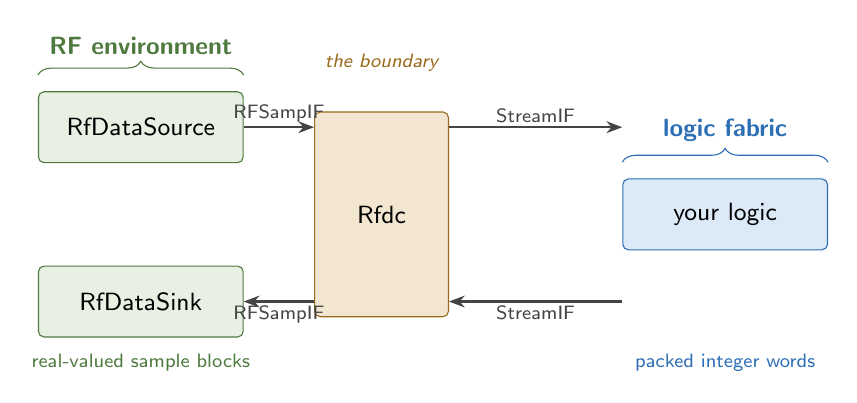
\begin{tikzpicture}[
  font=\sffamily\small,
  node distance=9mm,
  env/.style = {draw=envline, fill=envfill, rounded corners=2pt,
                minimum width=26mm, minimum height=9mm},
  cnv/.style = {draw=cnvline, fill=cnvfill, rounded corners=2pt,
                minimum width=17mm, minimum height=26mm},
  fab/.style = {draw=fabline, fill=fabfill, rounded corners=2pt,
                minimum width=26mm, minimum height=9mm},
  ln/.style  = {-{Stealth[length=2mm]}, draw=inkgray, thick},
  lbl/.style = {font=\sffamily\scriptsize, text=inkgray, inner sep=1.4pt},
]

% --- the three columns -------------------------------------------------------------------------
\node[env] (src)                        {RfDataSource};
\node[env, below=13mm of src] (snk)     {RfDataSink};
\node[cnv, right=22mm of $(src)!0.5!(snk)$] (rfdc) {Rfdc};
\node[fab, right=22mm of rfdc] (dut)    {your logic};

% --- the two paths -----------------------------------------------------------------------------
\draw[ln] (src.east)  -- node[lbl, above]        {RFSampIF}  (rfdc.west |- src);
\draw[ln] (rfdc.west |- snk) -- node[lbl, below] {RFSampIF}  (snk.east);

\draw[ln] (rfdc.east |- src) -- node[lbl, above] {StreamIF}  (dut.west |- src);
\draw[ln] (dut.west |- snk)  -- node[lbl, below] {StreamIF}  (rfdc.east |- snk);

% --- what each side carries --------------------------------------------------------------------
\node[lbl, below=1.5mm of snk.south, text=envline] {real-valued sample blocks};
\node[lbl, below=1.5mm of snk.south -| dut, text=fabline] {packed integer words};

% --- the braces: two domains, and the converter under neither ------------------------------------
\draw[decorate, decoration={brace, amplitude=5pt, raise=3pt}, draw=envline]
  ($(src.north west)+(0,1mm)$) -- ($(src.north east)+(0,1mm)$)
  node[midway, above=7pt, text=envline, font=\sffamily\small\bfseries] {RF environment};

\draw[decorate, decoration={brace, amplitude=5pt, raise=3pt}, draw=fabline]
  ($(dut.north west)+(0,1mm)$) -- ($(dut.north east)+(0,1mm)$)
  node[midway, above=7pt, text=fabline, font=\sffamily\small\bfseries] {logic fabric};

\node[lbl, above=13pt of rfdc.north, text=cnvline, font=\sffamily\scriptsize\itshape]
  {the boundary};

\end{tikzpicture}
\end{document}
